\documentclass[a4paper,10pt]{article}
\usepackage[utf8]{inputenc}

\usepackage{graphicx}
\usepackage{float}

% Packages to embbed Matlab code
\usepackage[framed,numbered,autolinebreaks,useliterate]{mcode}
\usepackage{url,textcomp}
\setlength{\parindent}{0pt}

%opening
\title{Homework 2 - Robot Dynamics and Control}
\author{Erivelton Gualter dos Santos}

\begin{document}

\date{}
\maketitle

\section*{Preliminary steps}

\begin{enumerate}
 \item Determine the slight difference between Matlab’satan2and the function shown inAppendix A of SHV.
\end{enumerate}

% Problem 1
\section{Problem}

Find the Euler angles equivalent to the following sequence ofrotations: Rotx($\frac{\pi}{2}$), Roty($-\pi$) (relative to $y_0$), Roty($\frac{\pi}{2}$) (relative to the current frame) and Rotz(-$\frac{\pi}{2}$) (relative toz0). Sketch all frames and verify that the Euler angles for the composite rotation work (if there are multiple solutions, show them all).

\hfill \break

The following figure illustrate the rotation by step-by-step:

\begin{figure}[H] \label{fig:frames}
 \centering
 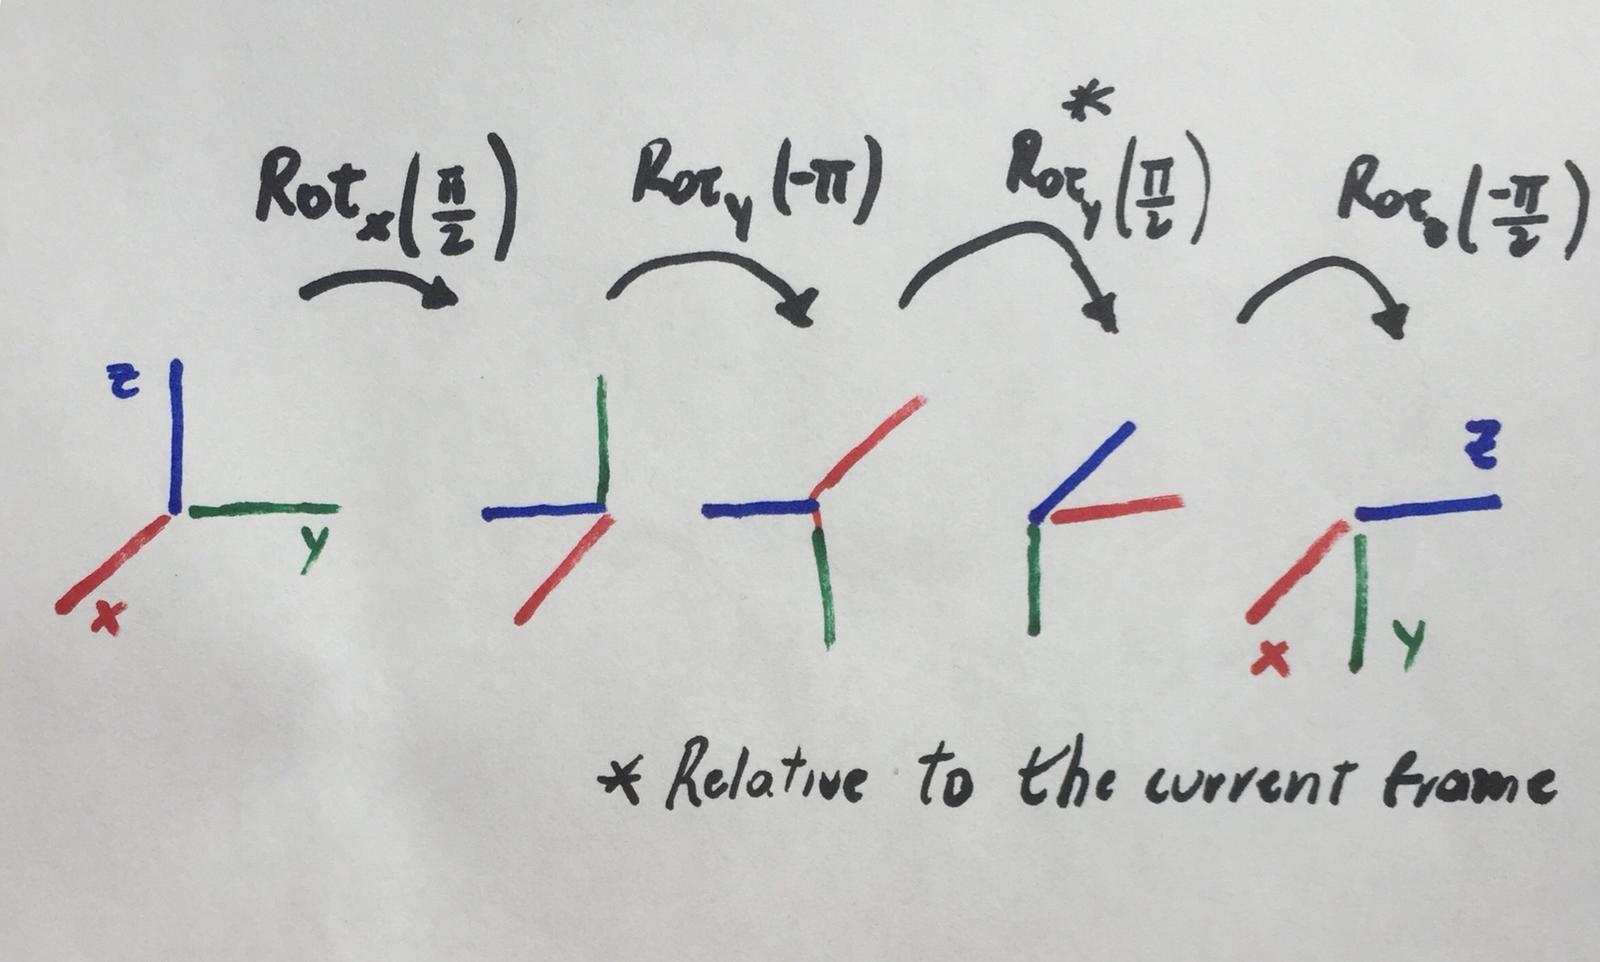
\includegraphics[width=0.7\linewidth]{pb1.jpeg}
 \caption{Snapshot of frames.}
\end{figure}

It is clearly that the last frame correspond to:

$$\left(\begin{array}{c} x'\\ y'\\ z' \end{array}\right)  = \left(\begin{array}{ccc} 1 & 0 & 0\\ 0 & 0 & 1\\ 0 & -1 & 0 \end{array}\right)\left(\begin{array}{c} x\\ y\\ z \end{array}\right) = \left(\begin{array}{c} x\\ z\\ -y \end{array}\right)$$

\begin{lstlisting}
%% Problem 1
R04 = Rotz(-sym(pi/2))*Roty(-sym(pi))*Rotx(sym(pi)/2)*Roty(sym(pi/2))

function out = Rotx(alpha)
%Rot_x: Basic rotation matrix about the x-axes 
out = [1 0 0 ; ...
    0 cos(alpha) -sin(alpha); ....
    0 sin(alpha) cos(alpha)]; 
end

function out = Roty(alpha)
%Rot_y: Basic rotation matrix about the y-axes 
out = [cos(alpha) 0 sin(alpha); ...
    0 1 0; ...
    -sin(alpha) 0 cos(alpha)]; 
end

function out = Rotz(alpha)
%Rot_z: Basic rotation matrix about the z-axes 
out = [cos(alpha) -sin(alpha) 0; ...
    sin(alpha) cos(alpha) 0; ...
    0 0 1]; 
end


\end{lstlisting}

% Problem 2
\section{Problem}

Consider the PP robot with spherical wrist shown in Fig. \ref{fig:5dof}. Consider all 3 d.o.f. of the spherical wrist to be concentric (zero lengths betweenjoints)


\begin{figure}[H] \label{fig:5dof}
 \centering
 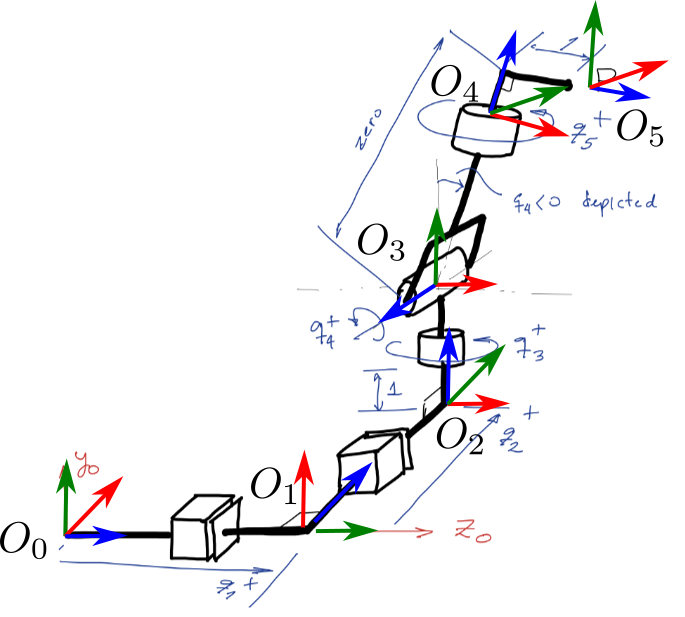
\includegraphics[width=0.7\linewidth]{5DOF.png}
 \caption{5-DOF robot with spherical wrist.}
\end{figure}


% Please add the following required packages to your document preamble:
% \usepackage{booktabs}
\begin{table}[H]
\caption{DH parameters for the 5-DOF manipulator.}
\begin{center}
\label{table:simulation}
\begin{tabular}{c c c c c} \hline
Link & $a_i$ & $\alpha_i$       & $d_i$ & $\theta_i$      \\ \hline \hline
1    & 0     & $\frac{\pi}{2}$  & $q_1$ & $\frac{\pi}{2}$ \\
2    & 0     & $\frac{\pi}{2}$  & $q_2$ & $\frac{\pi}{2}$ \\
3    & 0     & $\frac{\pi}{2}$  & $q_3$ & $q_3$           \\
4    & 0     & $\frac{-\pi}{2}$ & 0     & $q_4$           \\
$^a$     & $d_5$ & 0                & 0     & $q_5$           \\
5    & 0     & $\frac{\pi}{2}$  & 0     & $\frac{\pi}{2}$ \\ \hline
\end{tabular}
\end{center}
\centering
\footnotesize{$^a$ Intermediate frame.}\\
\end{table}

\begin{figure}[H] \label{fig:conf0}
 \centering
 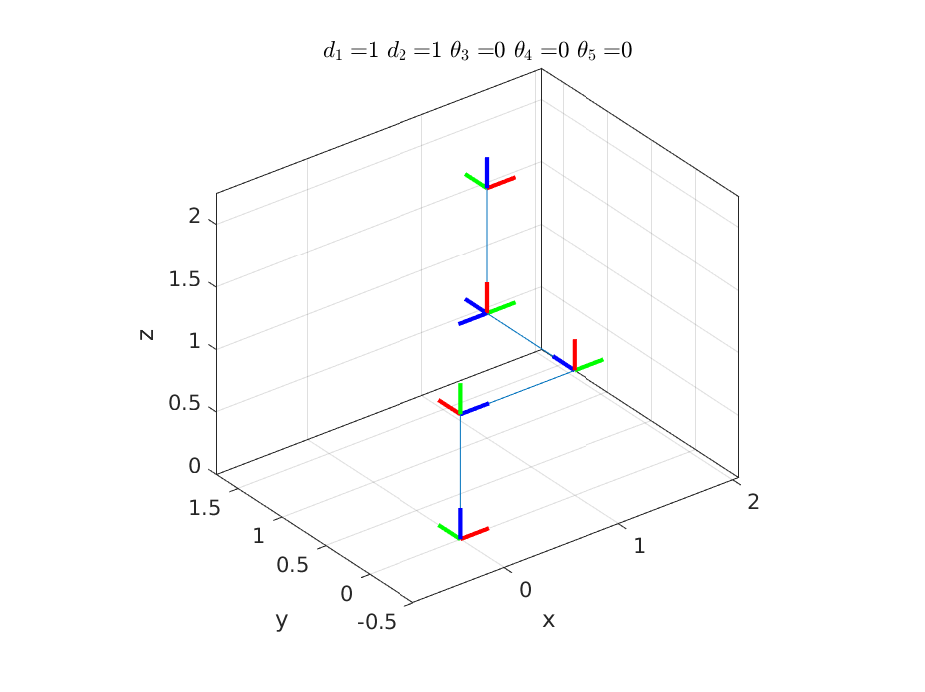
\includegraphics[width=0.7\linewidth]{configuration0.eps}
 \caption{Zero angle configuration.}
\end{figure}

\begin{figure}[H] \label{fig:conf1}
 \centering
 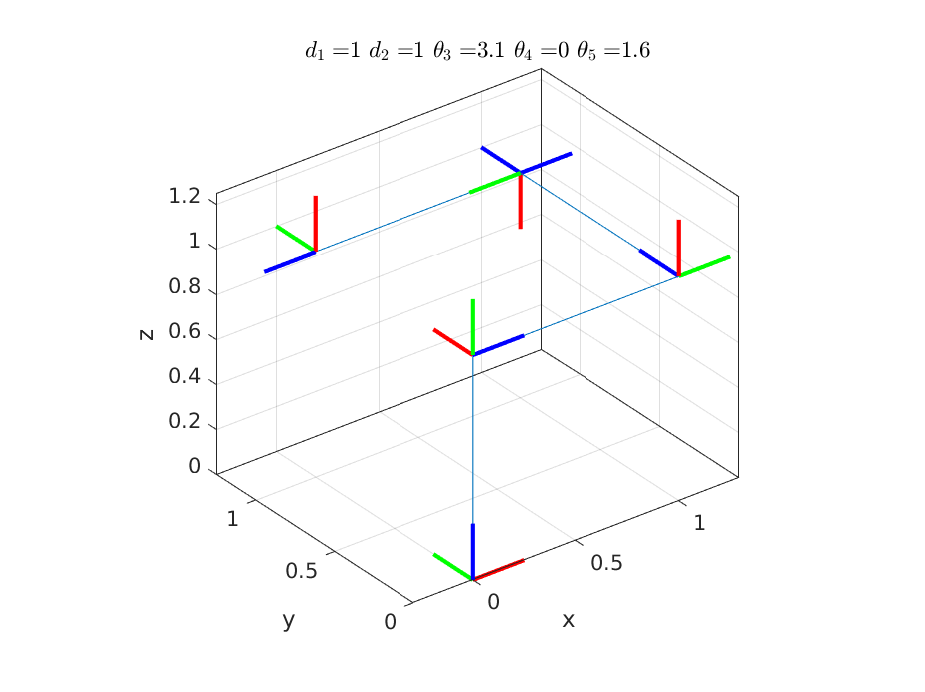
\includegraphics[width=0.7\linewidth]{configuration1.eps}
 \caption{``Easy'' configuration test \#1.}
\end{figure}

\begin{figure}[H] \label{fig:conf2}
 \centering
 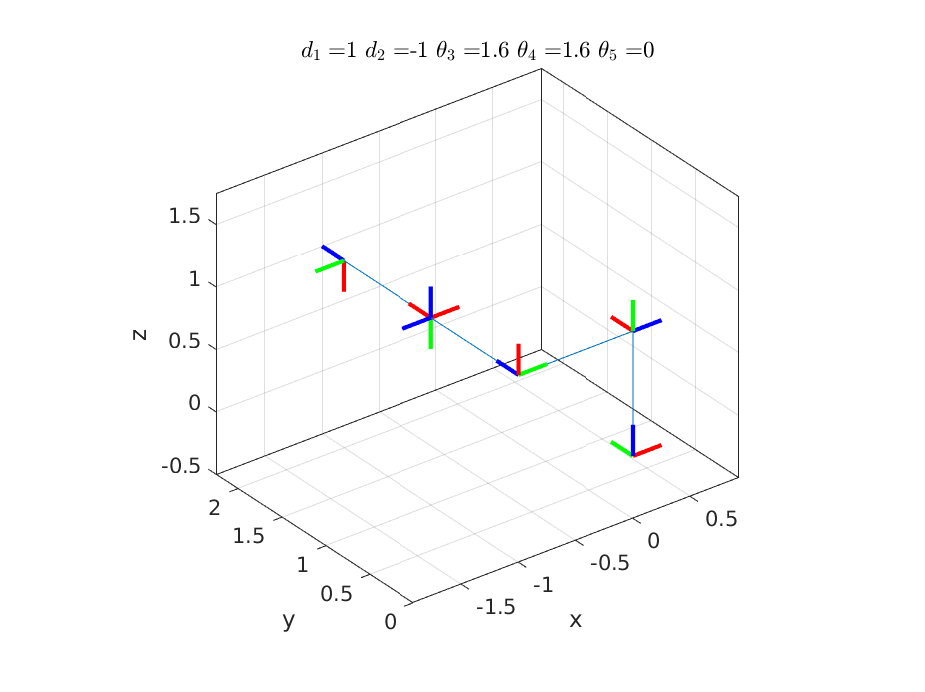
\includegraphics[width=0.7\linewidth]{configuration2.eps}
 \caption{``Easy'' configuration test \#2.}
\end{figure}

\begin{figure}[H] \label{fig:}
 \centering
 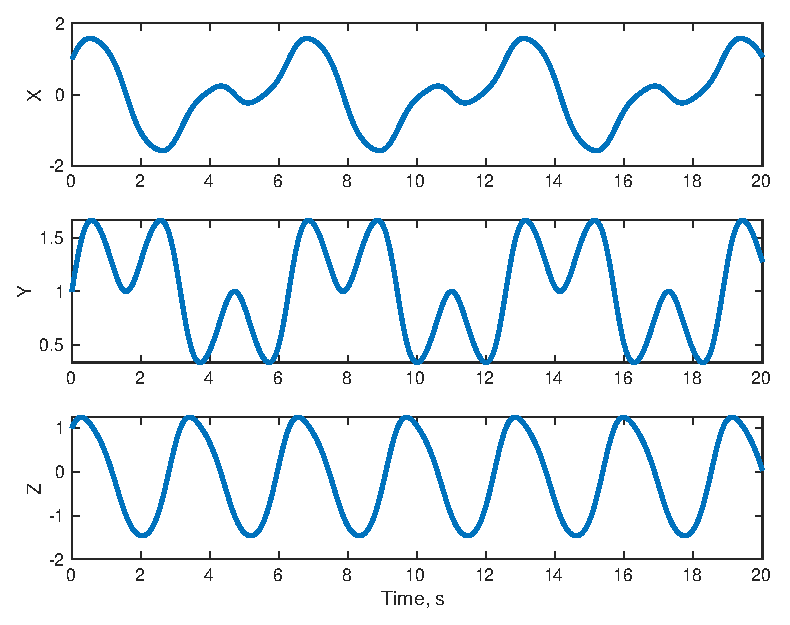
\includegraphics[width=0.7\linewidth]{EndETrajTime.eps}
 \caption{Position of End-Effector along the time.}
\end{figure}

\begin{figure}[H] \label{fig:}
 \centering
 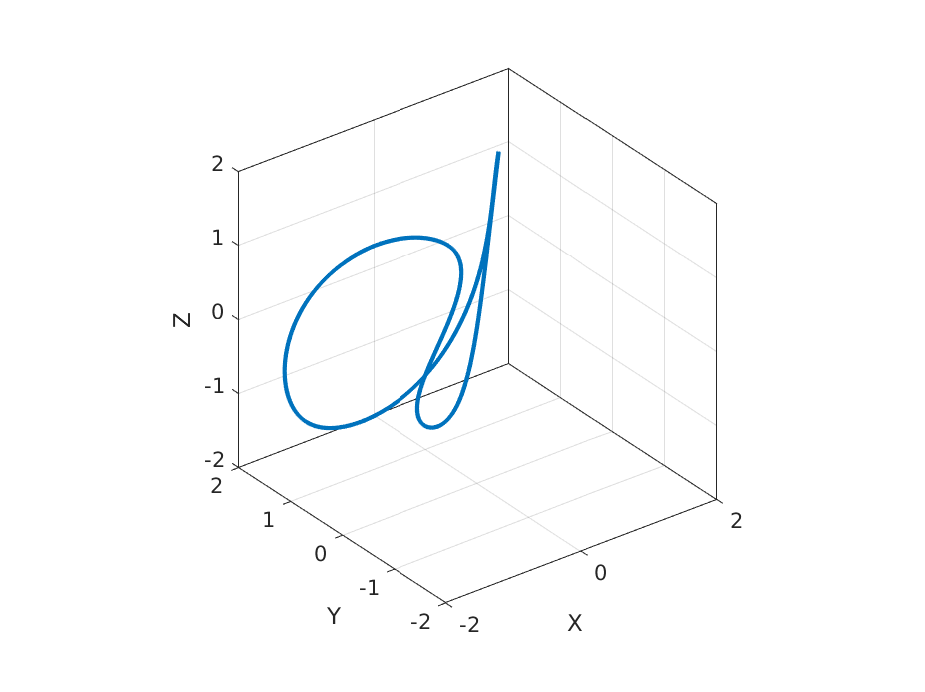
\includegraphics[width=0.7\linewidth]{EndETraj3D.eps}
 \caption{End-Effector trajectory on Space.}
\end{figure}

\end{document}



